\section{Lebenszeitmessungen}
	In diesem Versuchsteil soll die Lebenszeit von Zellen, die sich im angeregten Zustand befinden, ermittelt werden. Die Zellen sind dabei entweder mit CFP oder YFP bzw. mit CFP und YFP markiert. Der hierzu verwendete Laser ist ein gepulster $470\,$nm Laser mit einer Frequenz von $40\,$MHz. Zudem wurden noch zwei Avalanche-Photodioden mit entsprechenden Filterwürfeln benutzt. Wie dem Skript zu entnehmen ist, werden in Kanal 1 hauptsächlich CFP-Emissionen detektiert, wobei in Kanal 2 größtenteils YFP-Emissionen gemessen werden. Am Anfang des Versuchs wurde zunächst die instrument response function (kurz: IRF) gemessen. Dabei ergab sich folgendes Bild:
	\begin{figure}[h]
		\centering
		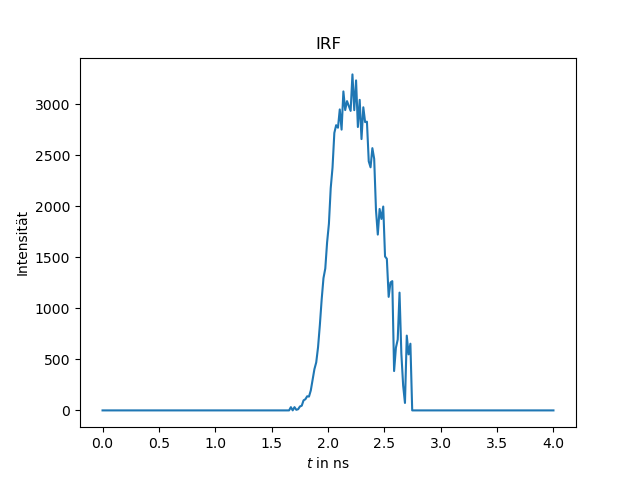
\includegraphics[width=7cm,height=5cm]{Auswertung-David/IRF-plot}
		\caption{Im Experiment gemessene IRF}
		\label{IRF}
	\end{figure}\\
	Anschließend wurde die Anzahl an detektierten Photonen über einem Zeitraum von ca. 2 Minuten gemessen und in Form eines Histogramms visualisiert. Das Histogramm einzelmarkierten Zellen wurde - im Bereich des exponentiellen Abfalls - durch einen single exponential fit genähert. Im Folgenden sind zwei Beispiele der daraus entstandenen Plots zu sehen.\\
	\begin{figure}[h]
		\begin{minipage}{.4\linewidth} % [b] => Ausrichtung an \caption
			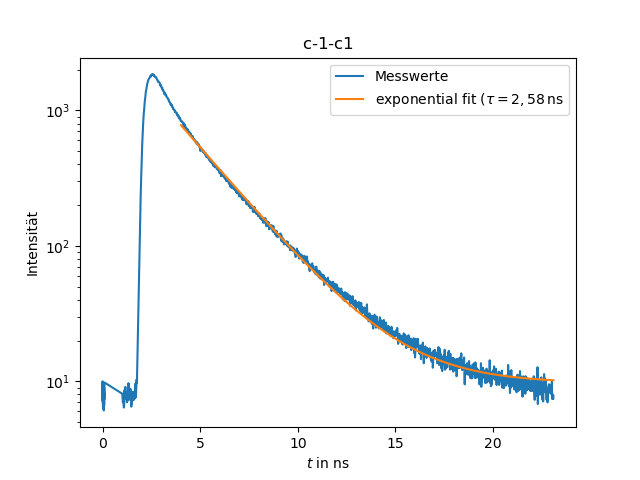
\includegraphics[width=\linewidth]{Auswertung-David/c-1-c1-plot}
			\caption{CFP-Signal in Kanal 1}
		\end{minipage}
		\hspace{.1\linewidth}% Abstand zwischen Bilder
		\begin{minipage}{.4\linewidth} % [b] => Ausrichtung an \caption
			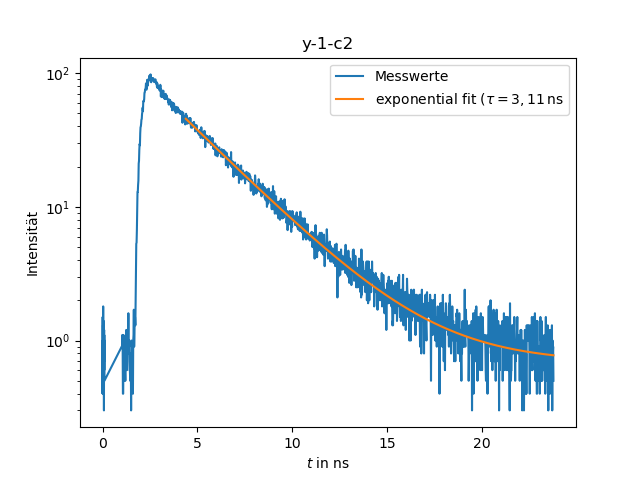
\includegraphics[width=\linewidth]{Auswertung-David/f-1-c2-plot}
			\caption{YFP-Signal in Kanal 2}
		\end{minipage}
	\end{figure}\\
Dadurch ergaben sich folgende Werte für die Lebenszeiten $\tau_{CFP}$ und $\tau_{YFP}$:\\
\begin{center} 
\begin{tabular}[c]{ccc}
	\hline
	 & $\tau_{CFP}$ in ns & $\tau_{YFP}$ in ns \\
	\hline
	Messung Nr. 1 & $2,58$ & $3,11$ \\
	Messung Nr. 2 & $2,51$ & $3,06$\\
	Messung Nr. 3 & $2,57$ & $3,03$\\
	\hline
	mittlere Lebensdauer & $2,55$ & $3,07$\\
	\hline
\end{tabular}\\
\end{center}
\newpage
Für die Bestimmung der Lebenszeiten der doppelt markierten Zellen wurde ein double exponential fit mit folgendem Ansatz genutzt:\\
\begin{equation}
N(t) = A_{1} \mathrm{e}^{-\frac{t}{\tau_1}}+A_{2} \mathrm{e}^{-\frac{t}{\tau_2}}
\end{equation}
Eine kleine Auswahl der Plots sah wie folgt aus:\\
\begin{figure}[h]
	\begin{minipage}{.4\linewidth} % [b] => Ausrichtung an \caption
		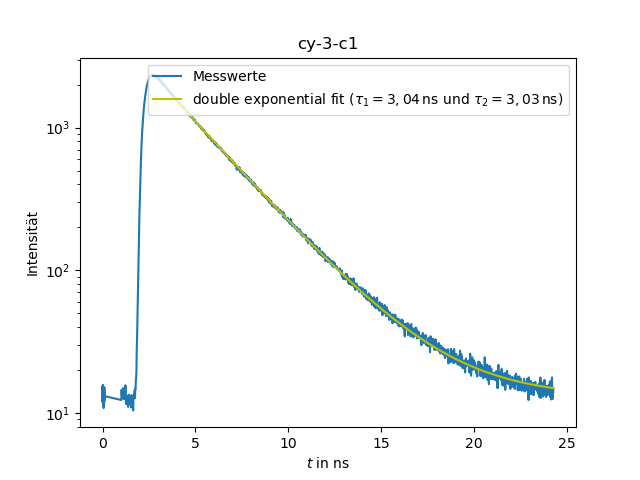
\includegraphics[width=\linewidth]{Auswertung-David/cy-3-c1-plot}
		\caption{CFP/YFP-Signal in \\Kanal 1}
	\end{minipage}
	\hspace{.1\linewidth}% Abstand zwischen Bilder
	\begin{minipage}{.4\linewidth} % [b] => Ausrichtung an \caption
		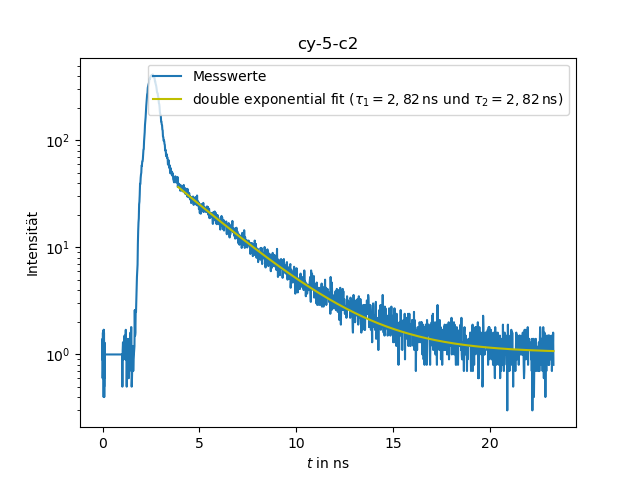
\includegraphics[width=\linewidth]{Auswertung-David/cy-5-c2-plot}
		\caption{CFP/YFP-Signal in \\Kanal 2}
	\end{minipage}
\end{figure}\\
Das Vorgehen zur Bestimmung der Lebenszeiten erfolgte analog zu oben und ergab folgende Werte:\\
\begin{center} 
	\begin{tabular}[c]{ccc}
		\hline
		& $\tau_{\mathrm{Kanal 1}}$ in ns & $\tau_{\mathrm{Kanal 2}}$ in ns \\
		\hline
		Messung Nr. 1 & $2,31$ & $2,94$ \\
		Messung Nr. 2 & $3,00$ & $2,66$ \\
		Messung Nr. 3 & $3,04$ & $2,83$ \\
		Messung Nr. 4 & $2,97$ & $2,86$ \\
		Messung Nr. 5 & $3,01$ & $2,82$ \\
		\hline
		mittlere Lebensdauer & $2,87$ & $2,82$\\
		\hline
	\end{tabular}\\
\end{center}
Hieraus lässt sich nun die FRET-Effizienz bestimmen:\\
\begin{equation}
E = 1-\frac{\tau_{CFP,\:FRET}}{\tau_{CFP,\:no\:FRET}}=-0,13
\end{equation}
Es fällt sofort auf, dass die Lebenszeit ohne FRET kleiner ist, als die Lebenszeit mit FRET, was zu einer negativen FRET-Effizienz führt und das wiederum ist physikalisch nicht möglich. \\
Im letzten Abschnitt dieses Versuchsteils soll die Messkurve durch eine Faltung der IRF mit einem exponential fit angenähert werden.\\
\newpage
Hierbei ergab sich folgendes Bild:\\
\begin{figure}[h]
	\centering
	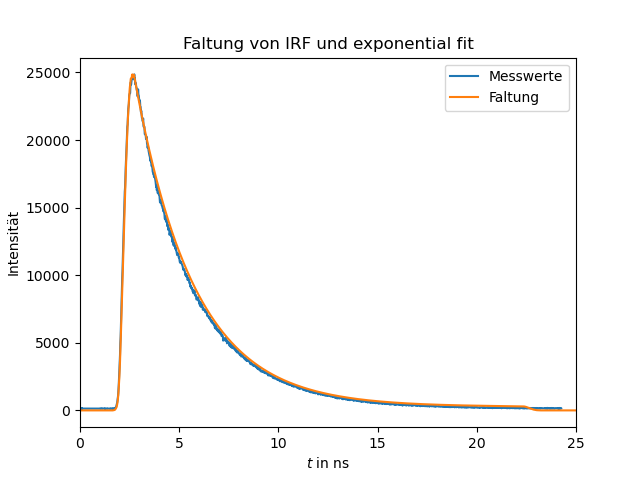
\includegraphics[width=9cm,height=7cm]{Auswertung-David/faltung-plot}
	\caption{Faltung der genäherten Exponentialfunktion mit der im Experiment ermittelten IRF}
	\label{Faltung von IRF und Exponentialfkt.}
\end{figure}\\
Anschließend wird die Exponentialfunktion noch mit einem Gauß-Fit der IRF gefaltet.  Für den Gauß-Fit ergaben sich eine Standardabweichung von $\sigma=0,21\,\mathrm{ns}$ und ein Erwartungswert von $\mu=2,26\,\mathrm{ns}$, woraus sich folgender Graph bestimmen ließ:
\begin{figure}[h]
	\centering
	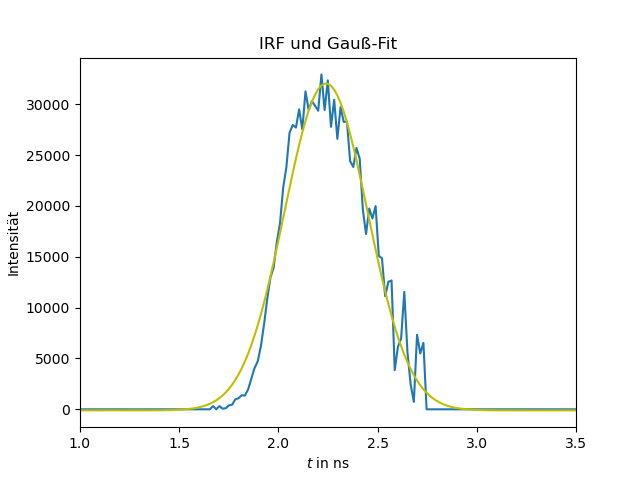
\includegraphics[width=9cm,height=7cm]{Auswertung-David/Gauss-fit-plot}
	\caption{Durch Gauß-Funktion genäherte IRF}
	\label{Gauss-Fit}
\end{figure}\\
\newpage
Durch die Faltung mit Gauß-Funktion und IRF entstand dieses Bild:
\begin{figure}[h]
	\centering
	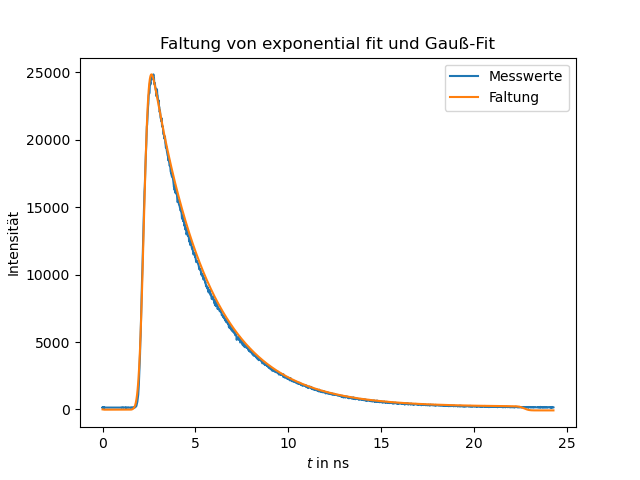
\includegraphics[width=9cm,height=7cm]{Auswertung-David/faltung-gauss-plot}
	\caption{Faltung von Gauß- und Exponentialfunktion}
	\label{Faltung mit Gauss-Fit}
\end{figure}\\
Die durch Faltung entstandene Funktion musste in beiden Fällen noch normiert werden, da bei der Faltung die Vorfaktoren - der miteinander gefalteten Funktionen - multipliziert wurden und die Faltung somit einige Größenordnungen über den Messwerten lag. Es fällt sofort auf, dass sich die Faltungen sehr gut an die Messkurve annähern und sich das Messsignal somit, durch die Faltung, ziemlich genau rekonstruieren lässt.
\newpage
\subsection{Abweichungen von Daten und Fits}
\begin{figure}[h]
	\centering
	\subfigure[Abweichung von Messwerten und Fit (cy-3-c1), berechnet mit np.cumsum($(y_{data}-y_{fit})^2$)]{
		\centering
		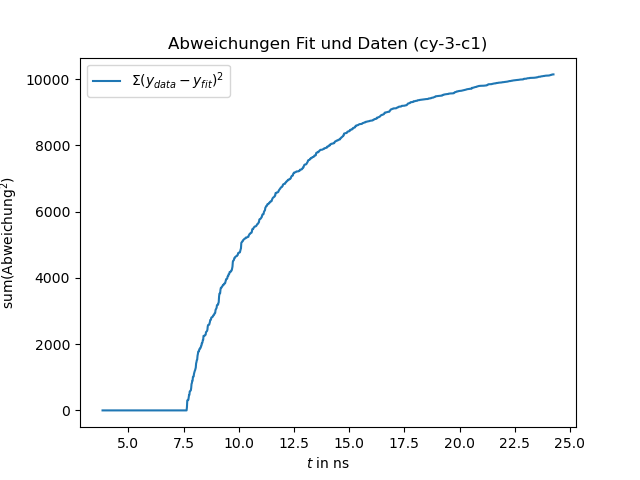
\includegraphics[width=0.3\textwidth]{Auswertung-David/Abweichungen_double_exp_fit_und_Daten_(cy-3-c1)}
		\label{fig:cy3c1}
	}
	\hfill
	\subfigure[Abweichung von Messwerten und Fit (cy-5-c2), berechnet mit np.cumsum($(y_{data}-y_{fit})^2$)]{
		\centering
		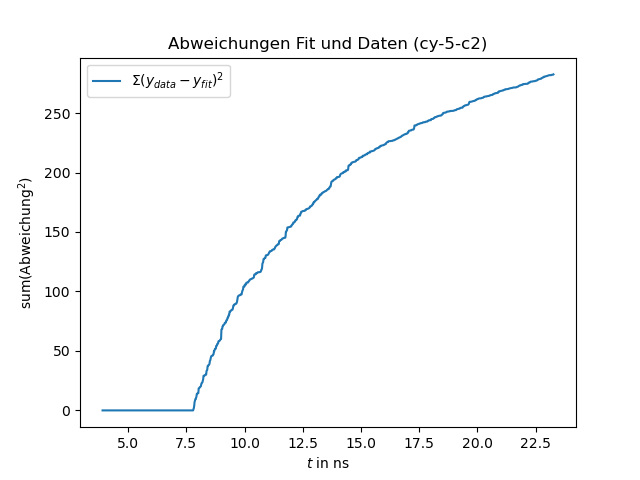
\includegraphics[width=0.3\textwidth]{Auswertung-David/Abweichungen_double_exp_fit_und_Daten_(cy-5-c2)}
		\label{fig:cy5c2}
	}
	\hfill
	\subfigure[Abweichungen von Faltung (IRF und Exp.) und Daten, berechnet mit np.cumsum($(y_{data}-y_{fit})^2$)]{
		\centering
		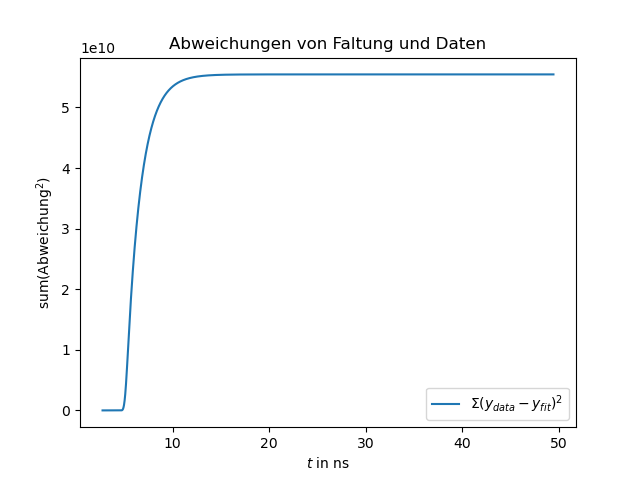
\includegraphics[width=0.3\textwidth]{Auswertung-David/Abweichungen_Faltung_und_Data}
		\label{fig:expIRF}
	}
	\hfill
	\subfigure[Abweichungen von Faltung (IRF und Gaußfkt.) und Daten, berechnet mit np.cumsum($(y_{data}-y_{fit})^2$)]{
		\centering
		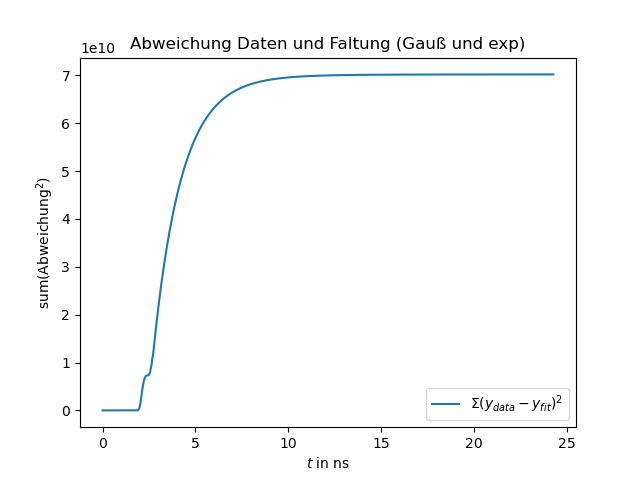
\includegraphics[width=0.3\textwidth]{Auswertung-David/Abweichungen_Gauss-Faltung_und_Data}
		\label{fig:gaussIRF}
	}
	\caption{Graphen der Summen der Abweichungen von Messwerten und Fits}
	\label{fig:abweichung}
\end{figure}